\lecture{5.2}{Bias--Variance Tradeoff}
\label{lec:5-2}

\subsection{Low Bias vs High Variance}

Bias and variance describe two different ways an estimator can perform poorly.
Suppose the target regression function is
\[
Q_0(a,w)=\E(Y\given A=a,W=w),
\]
and $\Qbar_n(a,w)$ is an estimator computed from a sample. At a fixed point
$(a,w)$, the bias is the difference between the average value of the estimator across
repeated samples and the truth:
\[
\Bias\{\Qbar_n(a,w)\}
=
\E\{\Qbar_n(a,w)\}-Q_0(a,w).
\]
The variance describes how much $\Qbar_n(a,w)$ changes from sample to sample:
\[
\Var\{\Qbar_n(a,w)\}
=
\E\left[
\left\{\Qbar_n(a,w)-\E\{\Qbar_n(a,w)\}\right\}^2
\right].
\]

An estimator can have low bias but high variance. For example, an estimator that uses
only people with covariates extremely close to $w$ may target the local conditional
mean accurately, but because it uses very few observations, its estimate can fluctuate
substantially across samples.

\subsection{High Bias vs Low Variance}

An estimator can also have high bias but low variance. A simple linear regression may
use the full sample and therefore produce stable estimates. But if the true regression
function is strongly nonlinear, the fitted line may systematically miss the truth.

\begin{keyidea}
Bias is systematic error from using a method that is too rigid or otherwise wrong.
Variance is random error from using a method that is too sensitive to the particular
sample. Good prediction requires balancing both.
\end{keyidea}

\subsection{Kernel Regression Intuition}

Kernel regression provides a concrete picture of the bias-variance tradeoff. Consider
estimating $\E(Y\given A=1,W=w_0)$. A simple local estimator is the uniform-kernel
estimator
\[
\Qbar_{n,h}(1,w_0)
=
\frac{\sum_{i=1}^nY_i\ind(A_i=1)\ind(|W_i-w_0|\le h/2)}
       {\sum_{i=1}^n\ind(A_i=1)\ind(|W_i-w_0|\le h/2)}.
\]
The tuning parameter $h>0$ is the bandwidth. The estimator averages outcomes among
treated individuals whose $W$ values fall inside a window of width $h$ centered at
$w_0$.

If $h$ is small, the estimator uses only very similar people. That reduces bias when
the regression function changes with $W$, but it increases variance because the
estimate is based on fewer observations. If $h$ is large, the estimator uses more
people. That reduces variance but may introduce bias by averaging over people who are
not very similar to $w_0$.

\subsection{Bandwidth Choice}

Bandwidth choice is a model selection problem. There is no universally best
bandwidth because the optimal choice depends on the unknown smoothness of the true
regression function and on the sample size. A very smooth true function can tolerate a
larger bandwidth. A highly curved true function requires a smaller bandwidth to avoid
oversmoothing.

\begin{figure}[H]
\centering
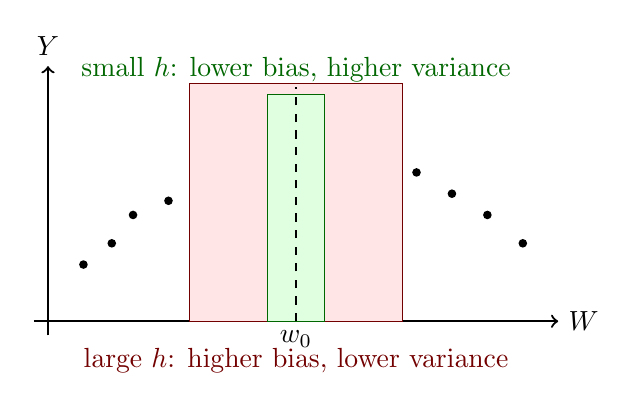
\begin{tikzpicture}[
  scale=.9,
  axis/.style={->, thick},
  pt/.style={circle, fill=black, inner sep=1.1pt},
  small/.style={fill=green!12, draw=green!40!black},
  large/.style={fill=red!10, draw=red!45!black}
]
\draw[axis] (-.2,0) -- (7.2,0) node[right] {$W$};
\draw[axis] (0,-.2) -- (0,3.6) node[above] {$Y$};
\foreach \x/\y in {.5/.8,.9/1.1,1.2/1.5,1.7/1.7,2.1/2.0,2.6/2.4,3.0/2.6,3.4/2.8,3.8/2.7,4.2/2.5,4.7/2.4,5.2/2.1,5.7/1.8,6.2/1.5,6.7/1.1}
  \node[pt] at (\x,\y) {};
\draw[large] (2.0,0) rectangle (5.0,3.35);
\draw[small] (3.1,0) rectangle (3.9,3.2);
\draw[dashed, thick] (3.5,0) -- (3.5,3.3);
\node[below] at (3.5,0) {$w_0$};
\node[green!40!black] at (3.5,3.55) {small $h$: lower bias, higher variance};
\node[red!45!black] at (3.5,-.55) {large $h$: higher bias, lower variance};
\end{tikzpicture}
\caption{The bandwidth controls how much information is borrowed across covariate values.}
\label{fig:ch5-bandwidth}
\end{figure}

\subsection{Parametric vs Semiparametric vs Nonparametric Methods}

Regression methods differ in how strongly they restrict the true regression function.

\begin{definition}[Parametric method]
A parametric regression method assumes that the regression function belongs to a
finite-dimensional family, such as
\[
\Qbar(a,w)=\beta_0+\beta_1a+\beta_2^\top w.
\]
\end{definition}

Parametric methods can have low variance because they impose strong structure, but
they can have high bias if the structure is wrong.

\begin{definition}[Semiparametric method]
A semiparametric method combines finite-dimensional components with flexible
components. For example,
\[
\Qbar(a,w)=\beta_0+\beta_1a+f(w)
\]
leaves the function $f$ unspecified or only weakly restricted.
\end{definition}

\begin{definition}[Nonparametric method]
A nonparametric method allows the regression function to become increasingly
flexible as the sample size grows. Examples include kernel regression, random
forests, neural networks, and certain spline or tree-based methods.
\end{definition}

The labels are less important than the practical consequence: different methods
borrow information in different ways and therefore occupy different points in the
bias-variance tradeoff.

\subsection{Unknown True Regression Function}

If the true regression function were known to be linear, a linear model would be a
natural choice. If the true function were known to have sharp interactions, a more
adaptive method would be needed. In practice, the true function is unknown.

This uncertainty is the motivation for Super Learning. Rather than choosing one
regression method because it is familiar, we pre-specify a library of plausible
candidate methods and use cross-validated risk to compare them.

\begin{estimationbox}
For causal estimation, model choice is not merely a prediction issue. Bias in
$\Qbar_n$ can bias g-computation; instability in $g_n$ can destabilize IPTW. The
next lectures develop a risk-based framework for choosing or combining nuisance
function estimators.
\end{estimationbox}
